\paragraph{\trCombinatorialFloerCohomology。}\label{sub:combinatorial-floer-cohomology}
设 $M$ 是一个二维的\trCorneredBoundary{}的\trExactSymplectic\trManifold。$M$ 中%
\trConnected{}的\trExact\trLagrange\trSubmanifold{}就是一条简单闭曲线 $S^1\cong L\subset%
\mathrm{int}(M)$，满足 $\int_L\theta=0$，其中 $\theta\in\Omega^1(M)$ 是\trSymplecticForm{}
$\omega$ 的\textbf{特异原函数}（distinguished primitive，若曲线有多个\trConnectedComponent，则每个分支上的积分都应为零）。%
注意，由\trStokes{}定理，这个条件排除了零\trHomology{}的曲线。取定一组彼此处于\trGeneralPosition{}的%
\trExact\trLagrange\trSubmanifold{} $\boldsymbol{L}=(L_1,\ldots,L_m)$；这就是说，任何%
两条都\trTransverse{}相交，并且没有三重交点。在 §9 的初步（\trUngraded{}且无符号）版本中%
定义\trFukayaCategory{} $\scr{F}(M)^{\mathrm{pr}}$ 时，可以取\trFloerDatum
\begin{equation}\label{eq:floer-data-trivial}
(H_{L_{i_0},L_{i_1}},\,J_{L_{i_0},L_{i_1}}),\qquad i_0<i_1
\end{equation}
为平凡的（$H=0$、$J=I_M$），而\trPerturbationDatum
\begin{equation}\label{eq:perturbation-data-trivial}
(K_{L_{i_0},\ldots,L_{i_d}},\,J_{L_{i_0},\ldots,L_{i_d}}),\qquad i_0<\cdots<i_d.
\end{equation}
亦然。
要验证这样做是允许的，涉及两个方面。第一方面由\cref{thm:automatic-regularity-surface}%
负责：它保证与 \eqref{eq:floer-data-trivial}、\eqref{eq:perturbation-data-trivial}%
相关联的\trFloer\trTrajectory{}与\trHolomorphicPolygon{}的诸\trModuliSpace{}都是%
\trRegular{}的；这些\trModuliSpace{}中没有常值映射，因为边界上的\trLagrange\trLabel{}
$L_{i_k}$ 彼此不同且处于\trGeneralPosition{}。第二点是 \eqref{eq:perturbation-data-trivial} 与%
\trPerturbationDatum{}的\trUniversal{}选取的\trConsistency{}条件\trCompatible，见%
\cref{sub:consistent-perturbation-data}。这是下述初等观察的推论：取一棵稳定的 $d$ 叶%
\trTree{} $T$，并对每个\trVertex{}取一个带\trLagrange\trLabel{}与\trStriplikeEnd{}的%
$|v|$ 点\trPointedDisc{} $S_v$。我们假设这些\trLabel{}是\trCompatible{}的，使得所有 $S_v$%
都能\trGluing{}成一个带\trLagrange\trLabel{}的 $(d{+}1)$ 点\trPointedDisc{} $S$。那么，%
若 $S$ 上的\trLabel{}是 $(L_{i_0},\ldots,L_{i_d})$（其中 $i_0<\cdots<i_d$），则每个分支 $S_v$%
上的\trLabel{}是它的一个有序子集，因而也具有同样的形式。
其次，假设 \eqref{eq:floer-data-trivial} 与 \eqref{eq:perturbation-data-trivial} 都已%
取为平凡，我们断言：\cref{sub:directed-subcategories} 意义下的\trDirected{}%
\trAinfty-子\trCategory{} $\scr{F}(\boldsymbol{L})^{\mathrm{pr},\to}\subset%
\scr{F}(M)^{\mathrm{pr}}$ 不依赖于\trComplexStructure{} $I_M$。换言之，对取定的%
$i_0<\cdots<i_d$ 与交点 $y_0\in L_{i_0}\cap L_{i_d}$、$y_k\in L_{i_{k-1}}\cap L_{i_k}$
（$1\le k\le d$），$\scr{M}^{d+1}(y_0,\ldots,y_d)$ 中\trIsolated{}点的数目在 $I_M$ 的%
\trHomotopy{}下不变。这可以用\trModuliSpace{}的一个直截了当的\trCobordism{}论证来证明；%
它可以看作 \cref{sub:homotopy-method} 中讨论的平凡情形：由于%
\cref{thm:automatic-regularity-surface}，\trParametrization{}的\trModuliSpace{}
$\scr{M}^{d+1}(y_0,\ldots,y_d)^{[0;1]}$ \trSmooth{}地\trFibration{}于 $[0;1]$ 之上，%
因而没有\trIsolated{}点，于是\cref{thm:homotopy-afunctor} 的\trAFunctor{}是恒等的。
在确立了 $\scr{F}(\boldsymbol{L})^{\mathrm{pr},\to}$ 原则上是\trTopology{}的之后，%
下一步是给出它的显式公式。这块地界早已被人踏遍（见本章开头的文献），所以我们从简。设%
$\Delta^{d+1}\subset\RR^2$ 是一个带\trOrientation{}的凸 $(d{+}1)$ 边形（$d=1$ 时这是%
一个二边形，即半月形），其\trCornerPoint{}与边按 $(d{+}1)$ 点\trPointedDisc{}的方式%
编号。给定点 $y_0,\ldots,y_d$ 如前，考虑由 $\Delta^{d+1}\to M$ 的\trSmooth{}%
\trImmersion{}（\trOrientation{}为正）组成的集合 $\mathrm{Imm}^{d+1}(y_0,\ldots,y_d)$，%
其中第 $k$ 个\trCornerPoint{}被映到 $y_k$，第 $k$ 条边被映到 $L_{i_k}$
（\cref{fig:immersed-polygon}）。我们坚持这些映射直到边界都必须是\trImmersion，
\begin{figure}[htbp]
\centering
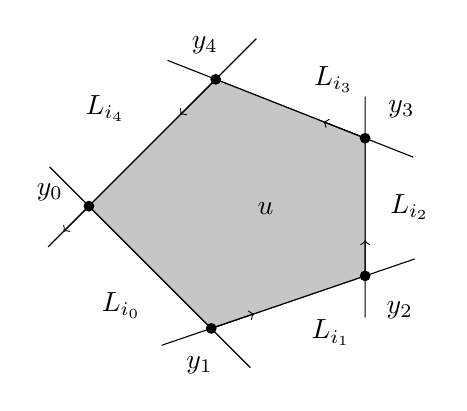
\begin{tikzpicture}[line cap=round,line join=round,scale=1.15]
\path (-1.9,0.15) coordinate (y0) (-0.55,-1.2) coordinate (y1)
      (1.15,-0.62) coordinate (y2) (1.15,0.9) coordinate (y3)
      (-0.5,1.55) coordinate (y4);
\path (y0)--(y1) coordinate[pos=-0.32] (e01a) coordinate[pos=1.32] (e01b);
\path (y1)--(y2) coordinate[pos=-0.32] (e12a) coordinate[pos=1.32] (e12b);
\path (y2)--(y3) coordinate[pos=-0.30] (e23a) coordinate[pos=1.30] (e23b);
\path (y3)--(y4) coordinate[pos=-0.32] (e34a) coordinate[pos=1.32] (e34b);
\path (y4)--(y0) coordinate[pos=-0.32] (e40a) coordinate[pos=1.32] (e40b);
\draw[thin] (e01a)--(e01b) (e12a)--(e12b) (e23a)--(e23b)
            (e34a)--(e34b) (e40a)--(e40b);
\fill[gray!45] (y0)--(y1)--(y2)--(y3)--(y4)--cycle;
\draw[thin] (y0)--(y1)--(y2)--(y3)--(y4)--cycle;
\path (y4)--(y0) coordinate[pos=1.20] (a0);
\path (y1)--(y2) coordinate[pos=0.28] (a1);
\path (y2)--(y3) coordinate[pos=0.26] (a2);
\path (y3)--(y4) coordinate[pos=0.28] (a3);
\path (y4)--(y0) coordinate[pos=0.28] (a4);
\draw[->,thin] (y0)--(a0);
\draw[->,thin] (y1)--(a1);
\draw[->,thin] (y2)--(a2);
\draw[->,thin] (y3)--(a3);
\draw[->,thin] (y4)--(a4);
\fill (y0) circle (1.7pt);
\fill (y1) circle (1.7pt);
\fill (y2) circle (1.7pt);
\fill (y3) circle (1.7pt);
\fill (y4) circle (1.7pt);
\node[anchor=east] at (-2.08,0.3) {$y_0$};
\node[anchor=north] at (-0.68,-1.4) {$y_1$};
\node[anchor=north west] at (1.28,-0.8) {$y_2$};
\node[anchor=south west] at (1.3,1.02) {$y_3$};
\node[anchor=south] at (-0.62,1.72) {$y_4$};
\node[anchor=north east] at (-1.22,-0.7) {$L_{i_0}$};
\node[anchor=north west] at (0.45,-1.0) {$L_{i_1}$};
\node[anchor=west] at (1.32,0.14) {$L_{i_2}$};
\node[anchor=south west] at (0.48,1.3) {$L_{i_3}$};
\node[anchor=south east] at (-1.4,0.98) {$L_{i_4}$};
\node at (0.05,0.12) {$u$};
\end{tikzpicture}
\caption{}\label{fig:immersed-polygon}
\end{figure}
这意味着每个\trCornerPoint{}附近的像是\trVertex{}处角度小于 $\pi$ 的一块楔形区域。%
$\Delta^{d+1}$ 的固定每个\trCornerPoint{}的\trDiffeomorphism{}群作用在%
$\mathrm{Imm}^{d+1}(y_0,\ldots,y_d)$ 上，而其\trQuotient{}可以等同于%
$\scr{M}^{d+1}(y_0,\ldots,y_d)$ 的零维部分。这事的证明如下：为方便起见，假设 $I_M$%
的选取使得在我们的曲线两两交点的附近都存在局部\trHolomorphic{}坐标，令这两条曲线成为 $\CC$ 中%
的实轴与虚轴。这不成问题，因为我们已经知道 $\scr{F}(\boldsymbol{L})^{\mathrm{pr},\to}$%
不依赖于 $I_M$（另一种办法是以多用一些分析为代价而取任意的 $I_M$，如 [114] 所示）。%
一个\trIndex{}论证 [43] 证明：任何\trIsolated{}的 $u\in\scr{M}^{d+1}(y_0,\ldots,y_d)$%
\footnote{译注：原书此处印作 $\scr{M}^{d+1}(x_0,\ldots,x_d)$；疑应为%
$\scr{M}^{d+1}(y_0,\ldots,y_d)$（与本节诸交点的记号一致）；此处径改。——译者注}%
都是\trImmersion，并且其像在诸无穷远点附近是楔形的。这一点，再辅以对 $u$ 沿诸%
\trStriplikeEnd{}的\trConvergence{}比的些许考虑，蕴含着可以把它\trCompactification{}%
为一个\trImmersion{} $\tilde{u}\colon\Delta^{d+1}\to M$。反方向——从一个%
\trImmersion{}出发构造\trHolomorphic{}映射——则依赖于如下事实：给 $\Delta^{d+1}$%
任意一个\trComplexStructure{}并挖去诸\trCornerPoint，剩下的便是一个 $(d{+}1)$%
\trPunctured\trDisk；这很容易归结为闭\trDisk{}的\trUniformization{}定理。
\begin{remark}\label{thm:generic-collection-combinatorial}
一个自然的问题是：$\scr{F}(M)^{\mathrm{pr}}$ 中由一个\trGeneric{}的组 $\boldsymbol{L}$%
构成的\trFullSubcategory{}是否也有一个组合式的描述。这看起来很可能，但答案应当比我们%
给出的这个复杂得多，原因在于交点处来自常值\trHolomorphicPolygon{}的贡献——在那里%
\cref{thm:automatic-regularity-surface} 失效（它们的\trModuliSpace{}维数超额：是%
\trSmooth{}的，但不\trRegular）。
\end{remark}
